\begin{frame}
	\frametitle{Concept}
	
	\begin{itemize}
		\item 2 minutes search budget
		\item 3 phases
	\end{itemize}
	
	\begin{figure}
		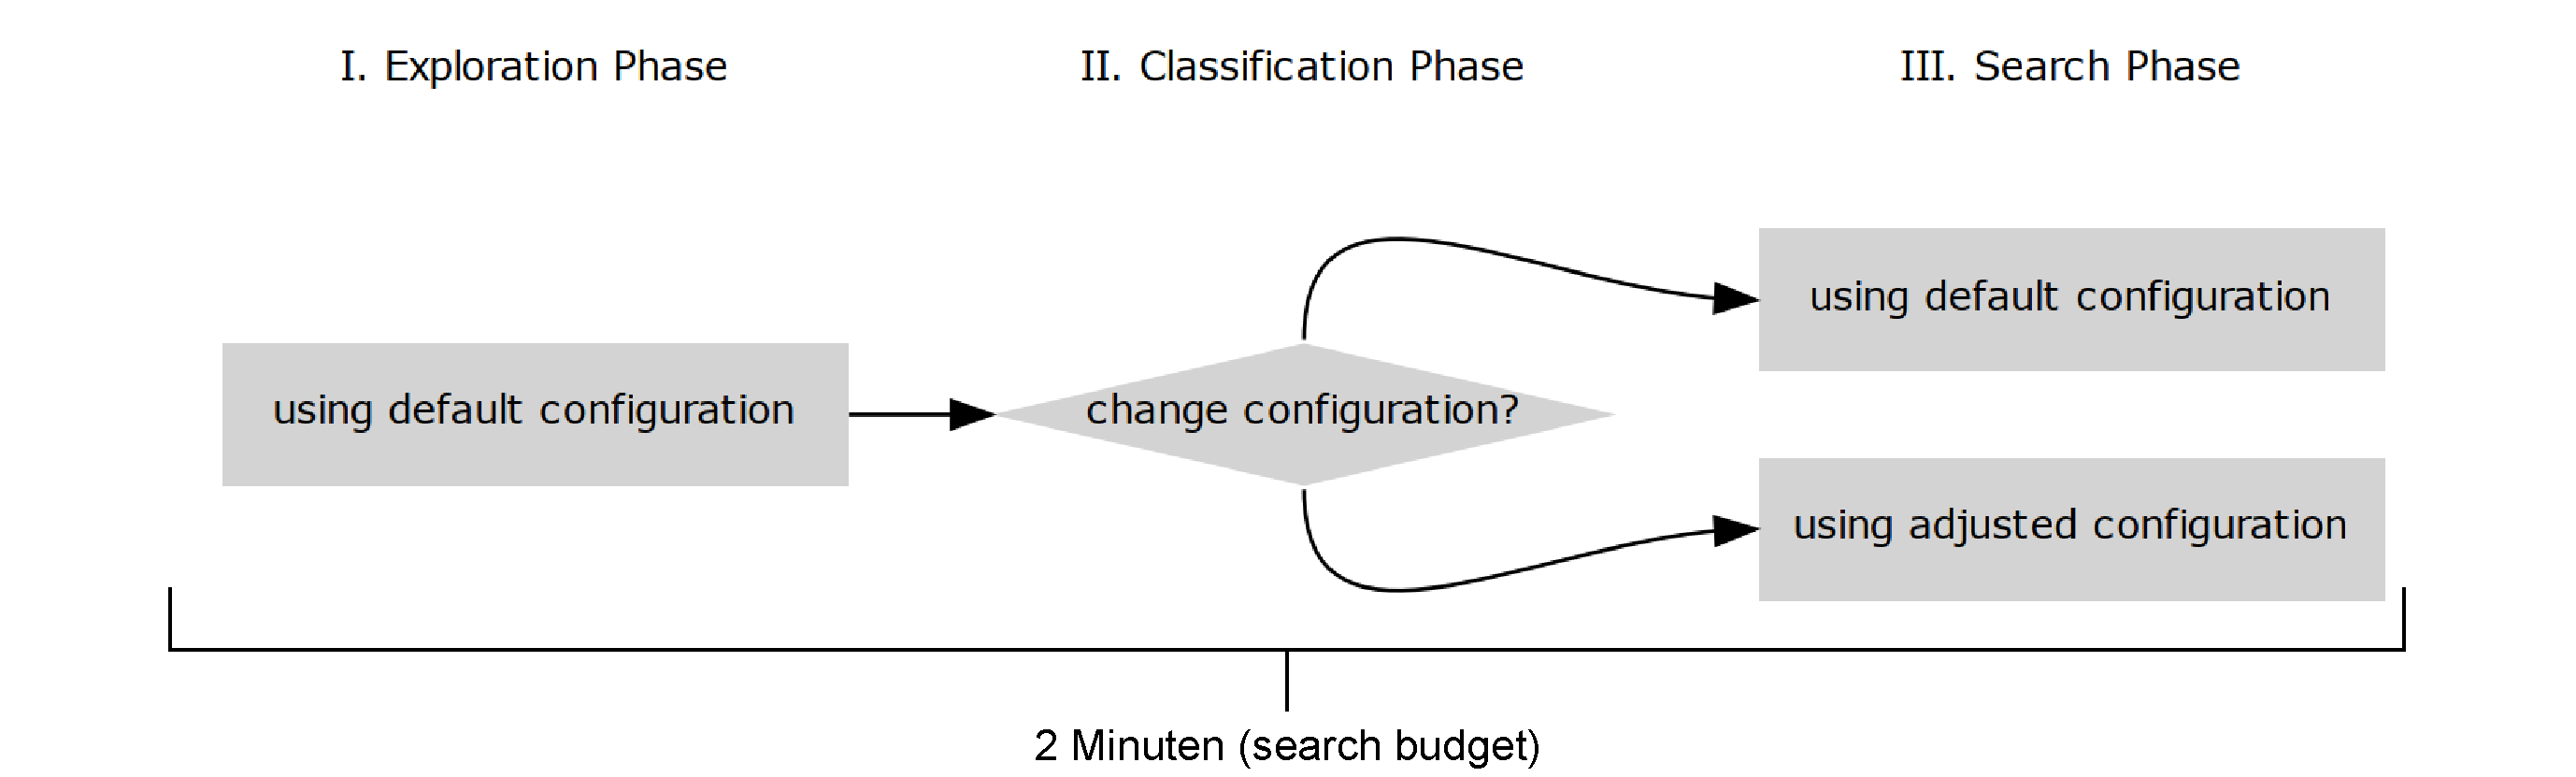
\includegraphics[width=1\textwidth]{figures/xxx}
	\end{figure}
	
\end{frame}

\begin{frame}
	\frametitle{Research questions}
	
	\begin{itemize}\setlength{\itemsep}{10pt}
		\item[$\blacksquare$] RQ 1. landscape features
		\item[$\blacksquare$] RQ 2. classification target
		\item[$\blacksquare$] RQ 3. classification model
		\item[$\blacksquare$] RQ 4. percentage of classification (POC)
		\item[$\blacksquare$] RQ 5. adjusted configuration
	\end{itemize}	

\end{frame}